From the different lab experiment conducted and further explained in the appendix, we decided the following settings for the 24h run. Our Bench scale reactor prototype operates 1 Rushton turbine and 1 Pitched blade at 280rpm, 35\si{\celsius}, with baffles in the vessel and cotton insulator outside. Cell concentration is monitored by 2 probes positioned 180º from each other and 2 sense leads 30º from the probe, 180º from each other. The following graphs display the data collected during the 24h run.

\begin{figure}[h!] %24h run
\begin{minipage}{0.3\textwidth}
    \centering
    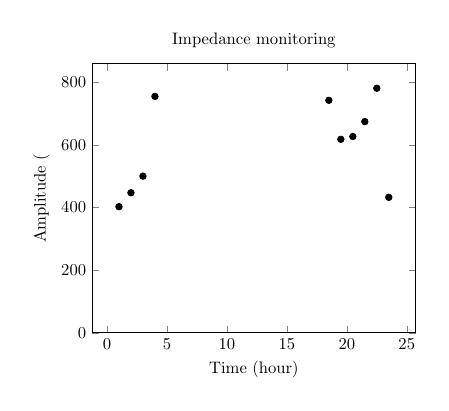
\begin{tikzpicture}[scale=0.6]
        \begin{axis}[xlabel=Time (hour), ymin=0, title={Impedance monitoring}, ylabel=Amplitude (\si{\milli\volt} ]
            \addplot[only marks] table{
                1	402.5
                2	447
                3	500
                4	754.5
                18.5	742
                19.5	617.5
                20.5	626.5
                21.5	674
                22.5	780.5
                23.5	432.5
            };
        \end{axis}
    \end{tikzpicture}
    \label{gr:24hImpedance}
\end{minipage}
\begin{minipage}{0.3\textwidth}
    \centering
    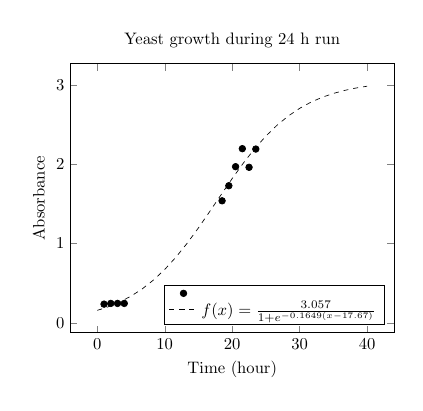
\begin{tikzpicture}[scale=0.6]
        \begin{axis}[title={Yeast growth during 24 h run}, ylabel=Absorbance , xlabel=Time (hour), legend pos = south east, domain=0:40]
            \addplot[only marks] table{
                1	0.236
                2	0.245
                3	0.245
                4	0.245
                18.5	1.538
                19.5	1.728
                20.5	1.968
                21.5	2.195
                22.5	1.96
                23.5	2.19
            };
            \addplot[dashed]{ 3.05695/(1+e^(-0.164931*(x-17.6678)) )};
        \addlegendentry{}
        \addlegendentry{$f(x) = \frac{3.057}{1+e^{-0.1649(x-17.67)}}$}   
        \end{axis}
    \end{tikzpicture}
\end{minipage}
\begin{minipage}{0.3\textwidth}
    \centering
    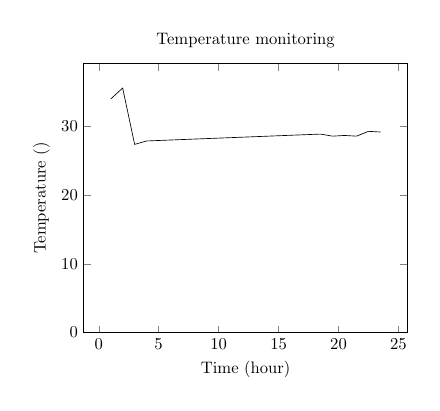
\begin{tikzpicture}[scale=0.6]
        \begin{axis}[title={Temperature monitoring}, ylabel=Temperature (\si{\celsius}) , xlabel=Time (hour), legend pos = south east, ymin=0]
            \addplot[] table{
            1	34.0
            2	35.6
            3	27.4
            4	27.9
            18.5	28.9
            19.5	28.6
            20.5	28.7
            21.5	28.6
            22.5	29.3
            23.5	29.2
            };
        \end{axis}
    \end{tikzpicture}
\end{minipage}
    \caption{From left to right: Impedance monitoring during 24h run; OD monitoring during 24h run; Temperature monitoring during 24h run.}
\end{figure}
